\section{Classical Algebraic Geometry}

\begin{frame}{Foray Into Algebraic Geometry}
    \begin{block}{Projective Space}
    Playing field is $n$\emph{-dimensional projective space}, $\PP^{n}$:
        $$ \PP^{n} := \{ (z_{0}, \ldots, z_{n}) \in \CC^{n} \} / (\vb{x} \sim \lambda \cdot \vb{y}), \quad \lambda \neq 0, $$
    that is, its elements consists of \emph{lines through the origin} in $\CC^{n}$.
    \end{block}
    

    \begin{center}
        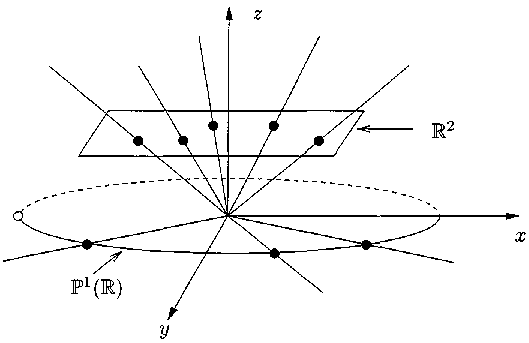
\includegraphics[height=0.35\textwidth, angle=0]{resources/projective-space}
    \end{center}

\end{frame}

\begin{frame}{Varieties}
    
    \emph{Varieties} are the objects studied in algebraic geometry, determined by the \emph{vanishing set}\footnote{from `\emph{Verschwindungsmenge}'} $V(-)$, for a system of polynomials.

    \begin{figure}
        \centering
        \begin{subfigure}[b]{0.475\textwidth}
            \centering
            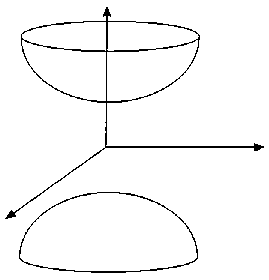
\includegraphics[width=0.35\textwidth]{resources/two-hyperboloid}
            \caption[]%
            {{\small $V(x^{2} + y^{2} - z^{2} + 1)$}}    
        \end{subfigure}
        \hfill
        \begin{subfigure}[b]{0.475\textwidth}  
            \centering 
            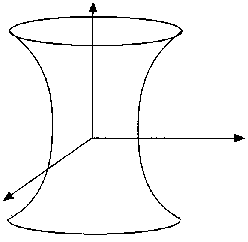
\includegraphics[width=0.35\textwidth]{resources/one-hyperboloid}
            \caption[]%
            {{\small $V(x^{2} + y^{2} - z^{2} - 1)$}}    
        \end{subfigure}
        \hfill
        \begin{subfigure}[b]{0.475\textwidth}   
            \centering 
            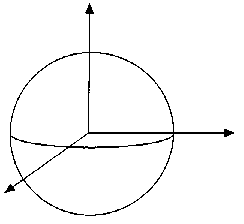
\includegraphics[width=0.35\textwidth]{resources/sphere}
            \caption[]%
            {{\small $V(x^{2} + y^{2} + z^{2} - 1)$}}    
        \end{subfigure}
        \hfill
        \begin{subfigure}[b]{0.475\textwidth}   
            \centering 
            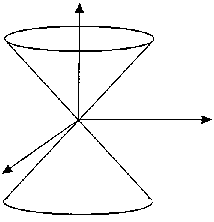
\includegraphics[width=0.35\textwidth]{resources/cone}
            \caption[]%
            {{\small $V(x^{2} + y^{2} - z^{2})$}}    
        \end{subfigure}
    \end{figure}

\end{frame}

\begin{frame}{Segre Varieties}
        \emph{Segre varieties} come from $\sigma: \PP^{n} \times \PP^{m} \ra \PP^{(n+1)(m+1) - 1}$, that sends $([X],[Y])$ to the pairwise products of their components:
            $$ \sigma : ([X_{1}, \ldots, X_{n+1}], [Y_{1}, \ldots, Y_{m+1}]) \mapsto [\ldots, X_{i}Y_{j}, \ldots ]. $$

        \begin{block}{Example - the Segre quadric surface}
        \vspace{-24pt}
        $$\sigma : \PP^{1} \times \PP^{1} \ra \PP^{3},\ ([X_{1}, X_{2}], [Y_{1}, Y_{2}]) \mapsto [ X_{1}Y_{1}, X_{1}Y_{2}, X_{2}Y_{1}, X_{2}Y_{2} ]. $$
        
        If we set $[ X_{1}Y_{1}, X_{1}Y_{2}, X_{2}Y_{1}, X_{2}Y_{2} ] =: [p_{11}, p_{12}, p_{21}, p_{22}]$, then:
        $$ \rightsquigarrow \det \begin{pmatrix} p_{11} & p_{12} \\ p_{21} & p_{22} \end{pmatrix} = 0 \iff \rank \begin{pmatrix} p_{11} & p_{12} \\ p_{21} & p_{22} \end{pmatrix} \leq 1. $$
        \end{block}
\end{frame}

\begin{frame}
    \begin{block}{Rulings}
    The Segre quadric surface has two families of lines in it, called \emph{rulings}. They are the images of $\sigma(\PP^{1} \times \{ \text{pt} \} )$ and $\sigma( \{ \text{pt} \} \times \PP^{1})$.
    \end{block}

    \begin{center}
        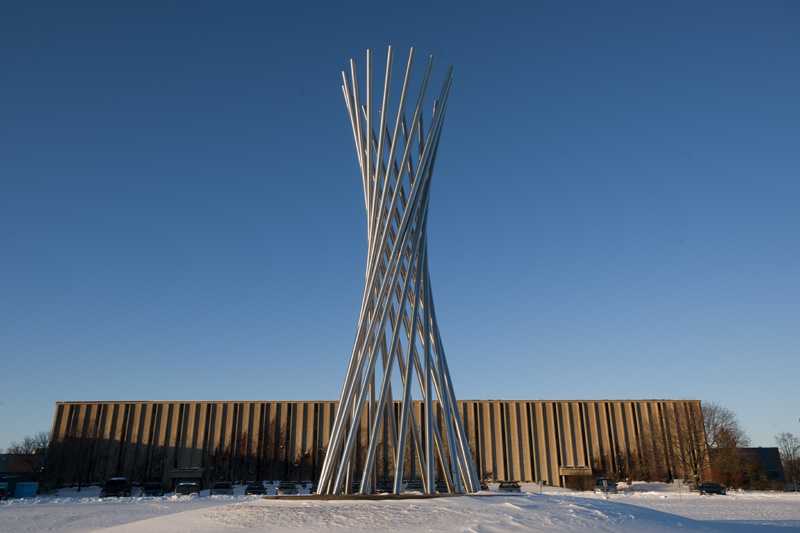
\includegraphics[height=0.35\textwidth]{resources/tractricious.jpg}
    \end{center}

\end{frame}

\begin{frame}{Manifold of Independence}

    \begin{itemize}
        \item Let $\Delta_{3} \subset \RR^{4}$, with vertices $A_{i} = e_{i}$. Denote a general point $p = (p_{ij}) \in \Delta_{3}$ by
        
        \begin{center}
        \begin{table}[]
        $p_{ij} = (p_{11}, p_{12}, p_{21}, p_{22}) =$ 
        \begin{tabular}{|l|l|}
        \hline
        $p_{11}$ & $p_{12}$ \\ \hline
        $p_{21}$ & $p_{22}$ \\ \hline
        \end{tabular}
        \end{table}
        \end{center}

    \item Fienberg & Gilbert have shown that the two rulings are given by
    \begin{center}
    \begin{table}[]
    \begin{tabular}{|c|c|}
    \hline
    $st$ & $s(1-t)$ \\ \hline
    $t(1-s)$ & $(1-s)(1-t)$ \\ \hline
    \end{tabular}
    $\quad (0 \leq s,t \leq 1).$
    \end{table}
    \end{center}
    
    \end{itemize}

    \begin{center}
        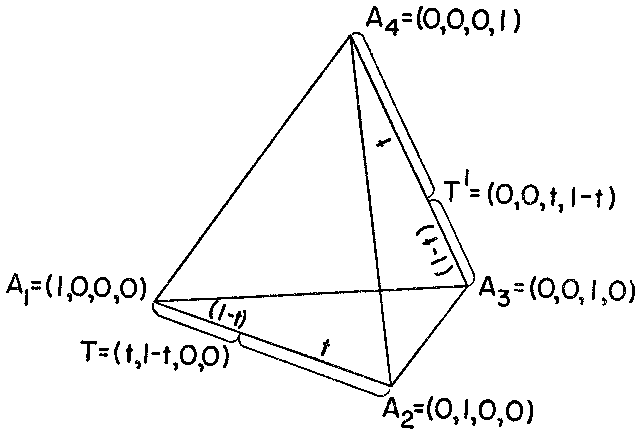
\includegraphics[height=0.25\textwidth]{resources/tetrahedron.pdf}
    \end{center}
    
\end{frame}

\begin{frame}
    TODO: FIGURE.
\end{frame}